\begin{figure}[H]
\centering

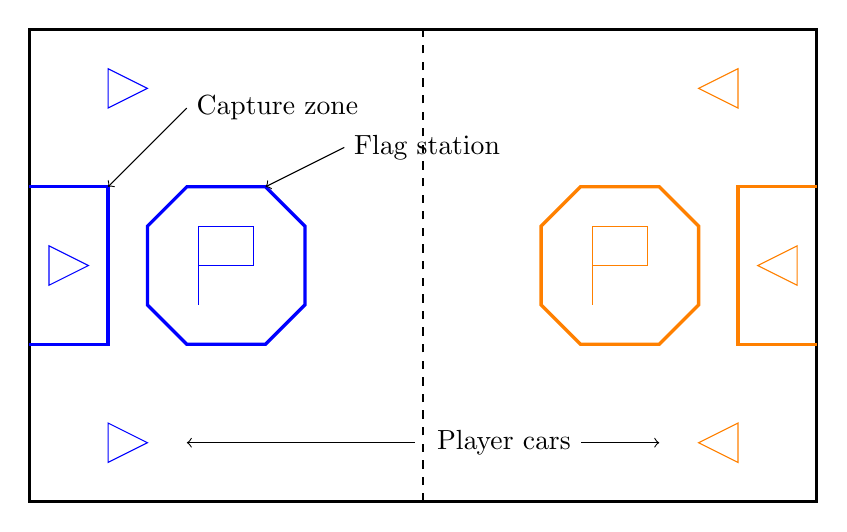
\begin{tikzpicture}

\draw[black, very thick] (-5, -3) rectangle (5, 3);
\draw[black, dashed] (0, -3) -- (0, 3);

% draw the blue base
\draw[blue, very thick] (-5, -1) -- (-4, -1) -- (-4, 1) -- (-5, 1);
\draw[blue, very thick] (-3.5, -0.5) -- (-3, -1) -- (-2, -1) -- (-1.5, -0.5) --
                        (-1.5, 0.5) -- (-2, 1) -- (-3, 1) -- (-3.5, 0.5) --
                        cycle;
\draw[blue] (-2.85, -0.5) -- (-2.85, 0.5) -- (-2.15, 0.5) -- (-2.15, 0) --
            (-2.85, 0);

% draw the blue cars
\draw[blue] (-4, 2.5) -- (-3.5, 2.25) -- (-4, 2) -- cycle;
\draw[blue] (-4.75, 0.25) -- (-4.25, 0) -- (-4.75, -0.25) -- cycle;
\draw[blue] (-4, -2.5) -- (-3.5, -2.25) -- (-4, -2) -- cycle;


% draw the orange base
\draw[orange, very thick] (5, -1) -- (4, -1) -- (4, 1) -- (5, 1);
\draw[orange, very thick] (3.5, -0.5) -- (3, -1) -- (2, -1) -- (1.5, -0.5) --
                          (1.5, 0.5) -- (2, 1) -- (3, 1) -- (3.5, 0.5) --
                          cycle;
\draw[orange] (2.15, -0.5) -- (2.15, 0.5) -- (2.85, 0.5) -- (2.85, 0) --
              (2.15, 0);

% draw the orange cars
\draw[orange] (4, 2.5) -- (3.5, 2.25) -- (4, 2) -- cycle;
\draw[orange] (4.75, 0.25) -- (4.25, 0) -- (4.75, -0.25) -- cycle;
\draw[orange] (4, -2.5) -- (3.5, -2.25) -- (4, -2) -- cycle;

% draw some labels
\draw[<-] (-4, 1) -- (-3, 2) node[anchor=west]{Capture zone};
\draw[<-] (-2, 1) -- (-1, 1.5) node[anchor=west]{Flag station};
\draw[<-] (3, -2.25) -- (2, -2.25) node[anchor=east]{Player cars};
\draw[<-] (-3, -2.25) -- (-0.1, -2.25);

\end{tikzpicture}

\caption{Diagram of the play field before release (not to scale). Obstacles will
be placed in the mid-field area to cause futher mayhem and shenanigans.}
\label{fig:play-field}
\end{figure}
